\documentclass[11pt,letterpaper]{article}


\usepackage[numbers,square]{natbib}
\renewcommand\cite[1]{(\citet{#1})}
\usepackage[hmargin=0.75in]{geometry}
\usepackage{color}
\usepackage{chemarr}
\usepackage{amssymb}
\usepackage{graphicx}
\usepackage{epstopdf}
\usepackage{caption}
\usepackage{subcaption}
\usepackage{placeins}
\usepackage{gensymb}
\usepackage{array}
%\usepackage{underscore}
\newcolumntype{L}{>{\arraybackslash}m{12cm}}
\usepackage{comment}
\usepackage{enumitem}

\title{Opt-IGFEM-2D: Developer's Guide}
\author{Marcus Hwai Yik Tan }
\date{Created on January 29th, 2016. Last revised on \today}

\begin{document}
\maketitle
\section{Structure of program}
\begin{figure}[!h]
\centering
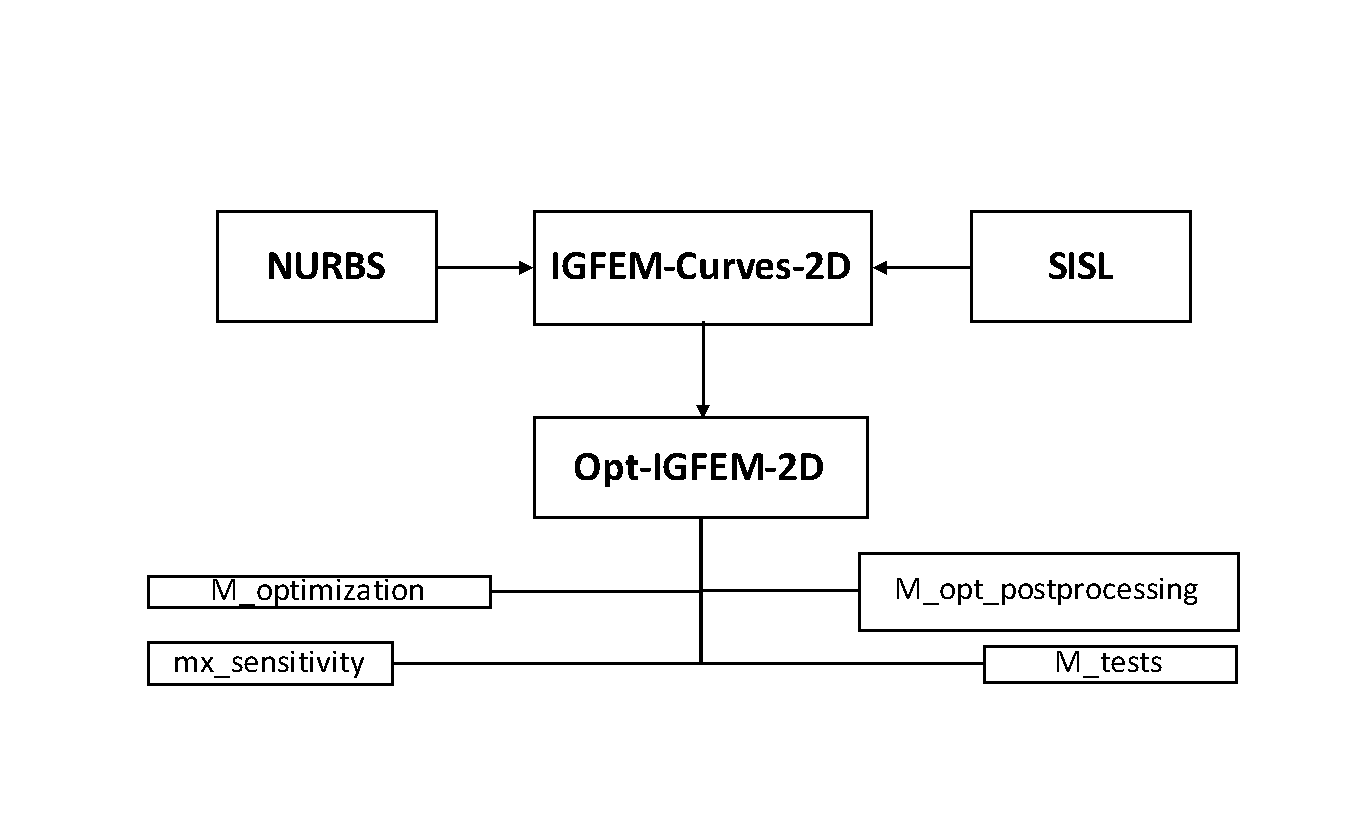
\includegraphics[width=\linewidth]{CodeStructure.pdf}
\caption{The directories (in bold) and subdirectories of the program. \label{fig_code_structure}}
\end{figure}

\section{Checking sensitivity analysis} 
The recommended first step to check the sensitivity analysis to is to compare the derivatives of the stiffness matrix and load vector wrt to a design parameter for the coarsest mesh with those obtained with finite difference. The derivatives resulting from the sensitivity analysis can be printed in MATLAB (but not output) by uncommenting the \texttt{\#define SHOW\_DK\_DP} directives in \texttt{sensitivity.h}, \texttt{assemble\_pseudo\_adjoint\_forces.cpp} and \texttt{IGFEM\_element\_pseudo\_adjoint\_forces.cpp}. One can then compare that derivatives with derivatives obtained from finite difference. The finite difference derivatives can be obtained by using the script \texttt{check\_DK\_DP.m}  in M\texttt{\_}tests (to be updated). 

The next step is to compare the derivatives of the objective function obtained from sensitivity analysis with the finite difference derivatives using \texttt{test\_objective\_derivatives.m} in  M\texttt{\_}tests
\section{Future Development}
The case of a moving channel inlet is currently under development for the Opt-IGFEM-3D project. Once this is done, the Opt-IGFEM-2D project would also be updated to include that case. 

\FloatBarrier    
\end{document}
